\documentclass[12pt]{report}
\usepackage[utf8]{inputenc}
\usepackage[english, russian]{babel}
\usepackage{listings}
\usepackage{graphicx}
\usepackage{float}
\graphicspath{{imgs/}}
\usepackage{amsmath,amsfonts,amssymb,amsthm,mathtools} 
\usepackage{pgfplots}
\usepackage{filecontents}
\usepackage{indentfirst}
\usepackage{eucal}
\usepackage{enumitem}
\frenchspacing

\usepackage{indentfirst} % Красная строка

\usetikzlibrary{datavisualization}
\usetikzlibrary{datavisualization.formats.functions}

\usepackage{amsmath}
\usepackage{fixltx2e}
\usepackage{caption}


\definecolor{bluekeywords}{rgb}{0,0,1}
\definecolor{greencomments}{rgb}{0,0.5,0}
\definecolor{redstrings}{rgb}{0.64,0.08,0.08}
\definecolor{xmlcomments}{rgb}{0.5,0.5,0.5}
\definecolor{types}{rgb}{0.17,0.57,0.68}

\usepackage{listings}
\lstset{language=[Sharp]C,
	captionpos=t,
	numbers=left, %Nummerierung
	numberstyle=\small, % kleine Zeilennummern
	frame=single, % Oberhalb und unterhalb des Listings ist eine Linie
	stepnumber=1,                   
	numbersep=5pt,                
	showspaces=false,
	tabsize=2,
	showtabs=false,
	breaklines=true,
	showstringspaces=false,
	breakatwhitespace=true,
	escapeinside={(*@}{@*)},
	commentstyle=\color{greencomments},
	morekeywords={partial, var, value, get, set},
	keywordstyle=\color{bluekeywords},
	stringstyle=\color{redstrings},
	basicstyle=\ttfamily\small,
}

\usepackage[left=1cm,right=1cm, top=1cm,bottom=2cm,bindingoffset=0cm]{geometry}
% Для измененных титулов глав:
\usepackage{titlesec, blindtext, color} % подключаем нужные пакеты
\definecolor{gray75}{gray}{0.75} % определяем цвет
\newcommand{\hsp}{\hspace{20pt}} % длина линии в 20pt
% titleformat определяет стиль
\titleformat{\chapter}[hang]{\Huge\bfseries}{\thechapter\hsp\textcolor{gray75}{|}\hsp}{0pt}{\Huge\bfseries}

\usepackage{array}
\newcommand{\head}[2]{\multicolumn{1}{>{\centering\arraybackslash}p{#1}}{#2}}

% plot
\usepackage{pgfplots}
\usepackage{filecontents}
\usetikzlibrary{datavisualization}
\usetikzlibrary{datavisualization.formats.functions}

\begin{document}
	%\def\chaptername{} % убирает "Глава"
	\thispagestyle{empty}
	\begin{titlepage}
		\noindent \begin{minipage}{0.15\textwidth}
			
\includegraphics[width=\linewidth]{b_logo}
		\end{minipage}
		\noindent\begin{minipage}{0.9\textwidth}\centering
			\textbf{Министерство науки и высшего образования Российской Федерации}\\
			\textbf{Федеральное государственное бюджетное образовательное учреждение высшего образования}\\
			\textbf{~~~«Московский государственный технический университет имени Н.Э.~Баумана}\\
			\textbf{(национальный исследовательский университет)»}\\
			\textbf{(МГТУ им. Н.Э.~Баумана)}
		\end{minipage}
		
		\noindent\rule{18cm}{3pt}
		\newline\newline
		\noindent ФАКУЛЬТЕТ $\underline{~~~~~~~~~~~~~~~~~~~~~~~~~~~~~~~\text{«Информатика и системы управления»}~~~~~~~~~~~~~~~~~~~~~~~~~~~~~~~~~~~~~}$ \newline\newline
		\noindent КАФЕДРА $\underline{~~~~~~~~~~~~~\text{«Программное обеспечение ЭВМ и информационные технологии»}~~~~~~~~~~~~~~~~~~~~~~~}$\newline\newline\newline\newline\newline\newline\newline\newline\newline\newline\newline
		
		
		\begin{center}
			\noindent\begin{minipage}{1.3\textwidth}\centering
				\Large\textbf{  Отчет по лабораторной работе №1}\newline
				\textbf{по дисциплине \newline "Моделирование"}\newline\newline
			\end{minipage}
		\end{center}
		
		\noindent\textbf{Тема} $\underline{\text{Изучение функций распределения и функций плотности распределения случайных чисел}}$\newline\newline
		\noindent\textbf{Вариант} $\underline{\text{15 (3)}}$\newline\newline
		\noindent\textbf{Студент} $\underline{\text{Малышев И. А.}}$\newline\newline
		\noindent\textbf{Группа} $\underline{\text{ИУ7-71Б}}$\newline\newline
		\noindent\textbf{Оценка (баллы)} $\underline{\text{~~~~~~~~~~~~~~~~~~~~~~~~~~~}}$\newline\newline
		\noindent\textbf{Преподаватель: } $\underline{\text{Рудаков И. В.}}$\newline\newline\newline
		
		\begin{center}
			\vfill
			Москва~---~\the\year
			~г.
		\end{center}
	\end{titlepage}
	
	
	\setcounter{page}{2}

\chapter{Задание}
Реализовать программу для построения графиков функций и плотности для следующих распределений: 

\begin{itemize}
	\item равномерное распределение
	\item распределение Пуассона
\end{itemize}

\chapter{Решение}
\section{Общий вид функций}

Функция равномерного распределения имеет следующий вид:

\begin{equation*}
	F_X(x) = 
	\begin{cases}
		0, x < a \\
		\resizebox{.045\hsize}{!}{$\frac{x - a}{b - a}$}, a \leqslant x < b \\
		1, x \geqslant b
	\end{cases}
\end{equation*}

Функция плотности равномерного распределения имеет следующий вид:

\begin{equation*}
	f_X(x) = 
	\begin{cases}
		0, x \notin [a, b] \\
		\resizebox{.04\hsize}{!}{$\frac{1}{b - a}$}, x \in [a, b] \\
	\end{cases}
\end{equation*}

Функция распределения Пуассона имеет следующий вид:

\begin{equation*}
	F_X(x) = e^{-\lambda}\sum_{i=0}^{k}{\frac{\lambda^i}{i!}}
\end{equation*}

Функция плотности распределения Пуассона имеет следующий вид:

\begin{equation*}
	f_X(x) = e^{-\lambda}\frac{\lambda^k}{k!}
\end{equation*}

\section{Листинг}

Далее представлен фрагмент программы, выполняющий поставленнуое задание.

\begin{lstlisting}
public interface IDistribution
{
	double CDF(double x);
	double PMF(double x);
}

public class UniformDistribution : IDistribution
{
	double a, b;
	
	public UniformDistribution(double a, double b)
	{
		if (b > a)
		{
			this.a = a;
			this.b = b;
		}
		else 
			throw new ArgumentException("a >= b");
	}
	
	public double CDF(double x)
	{
		if (x >= b)
			return 1.0;
		else if (x < a)
			return 0.0;
		else
			return (x - a) / (b - a);
	}
	
	public double PMF(double x)
	{
		if (x > a && x < b)
			return 1.0 / (b - a);
		else
			return 0.0;
	}
}

public class PoissonDistribution : IDistribution
{
	double lambda;
	
	public PoissonDistribution(double lambda)
	{
		if (lambda > 0.0)
			this.lambda = lambda;
		else
			throw new ArgumentException("Lambda <= 0");
	}
	
	public double CDF(double x)
	{
		double sum = 0;
		int k = (int)Math.Floor(x);
		
		for (int i = 0; i <= k; i++)
			sum += Math.Pow(lambda, i) / Factorial(i);
		
		return Math.Exp(-lambda) * sum;
	}
	
	public double PMF(double x)
	{
		int k = (int)Math.Floor(x);
		return (Math.Exp(-lambda) * Math.Pow(lambda, k)) / Factorial(k);
	}
}
\end{lstlisting}

\section{Результаты работы}

На рисунках \ref{img:ui1}-\ref{img:ui2} представлен пользовательский интерфейс программы в режиме построения графиков функций для равномерного распределения и в режиме построения графиков функций для распределения Пуассона.

\begin{figure}[H]
	\begin{center}
		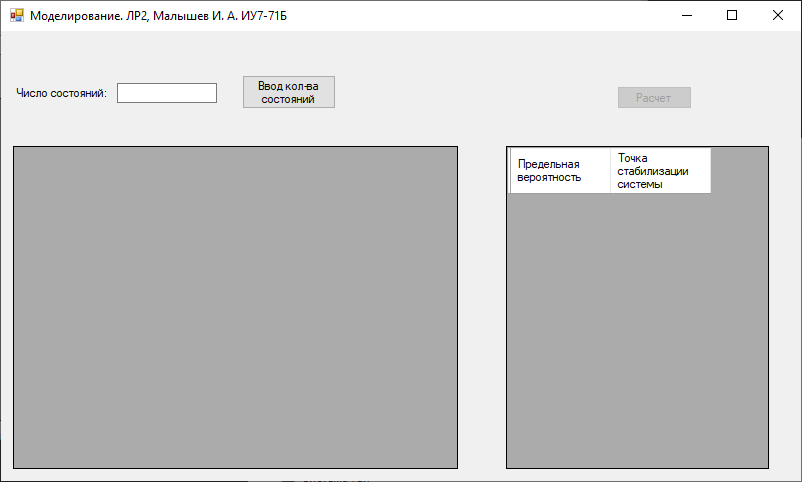
\includegraphics[scale=0.6]{imgs/ui1.png}
	\end{center}
	\caption{Пользовательский интерфейс программы в режиме построения графиков функций для равномерного распределения.}
	\label{img:ui1}
\end{figure}

\begin{figure}[H]
	\begin{center}
		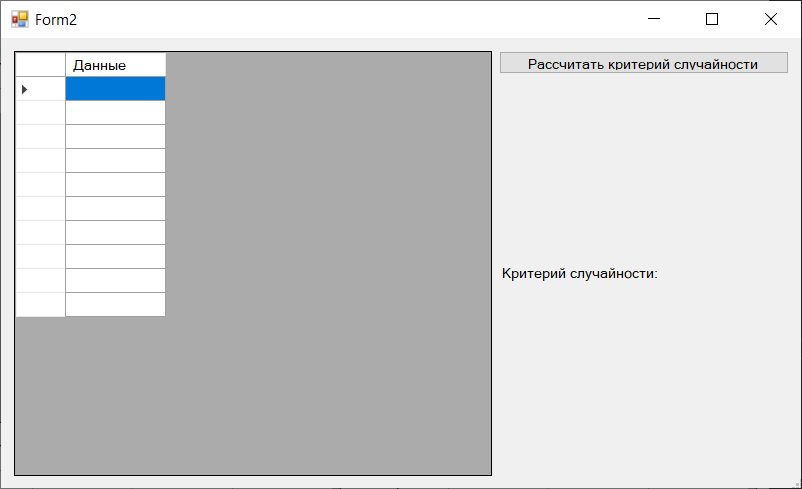
\includegraphics[scale=0.6]{imgs/ui2.png}
	\end{center}
	\caption{Пользовательский интерфейс программы в режиме построения графиков функций для распределения Пуассона.}
	\label{img:ui2}
\end{figure}

На рисунках \ref{img:uni1}-\ref{img:uni2} представлены примеры работы программы при построении графиков функции равномерного распределения и функции плотности равномерного распределения с разными значениями параметров $a$ и $b$.

\begin{figure}[H]
	\begin{center}
		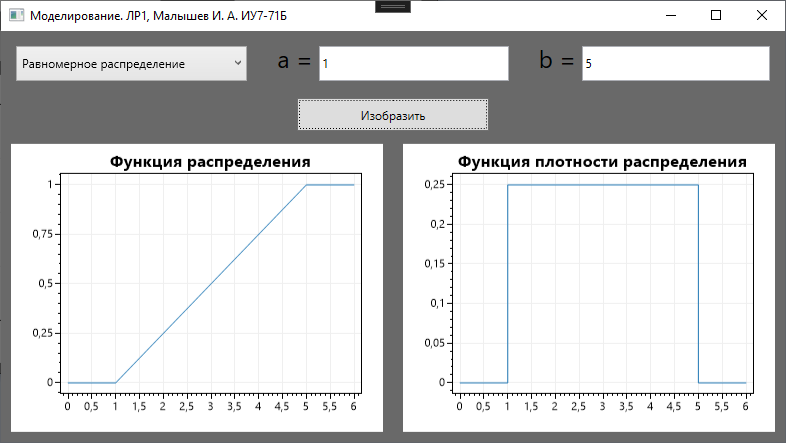
\includegraphics[scale=0.6]{imgs/uni1.png}
	\end{center}
	\caption{Пример работы программы со значениями парамеров $a = 1$ и $b = 5$.}
	\label{img:uni1}
\end{figure}

\begin{figure}[H]
	\begin{center}
		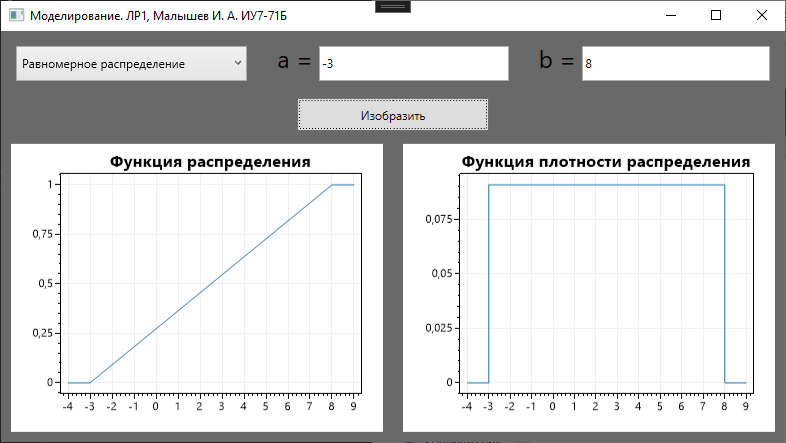
\includegraphics[scale=0.6]{imgs/uni2.png}
	\end{center}
	\caption{Пример работы программы со значениями парамеров $a = -3$ и $b = 8$.}
	\label{img:uni2}
\end{figure}

На рисунках \ref{img:pois1}-\ref{img:pois2} представлены примеры работы программы при построении графиков функции распределения Пуассона и функции плотности распределения Пуассона с разными значениями параметра $\lambda$.

\begin{figure}[H]
	\begin{center}
		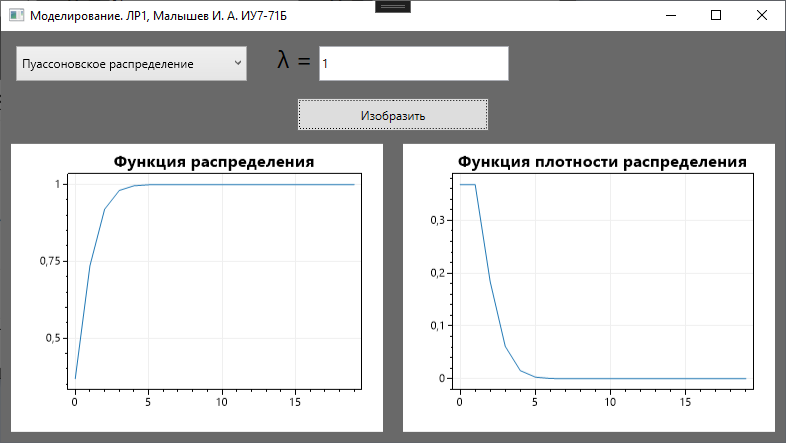
\includegraphics[scale=0.6]{imgs/pois1.png}
	\end{center}
	\caption{Пример работы программы со значением парамера $\lambda = 1$.}
	\label{img:pois1}
\end{figure}

\begin{figure}[H]
	\begin{center}
		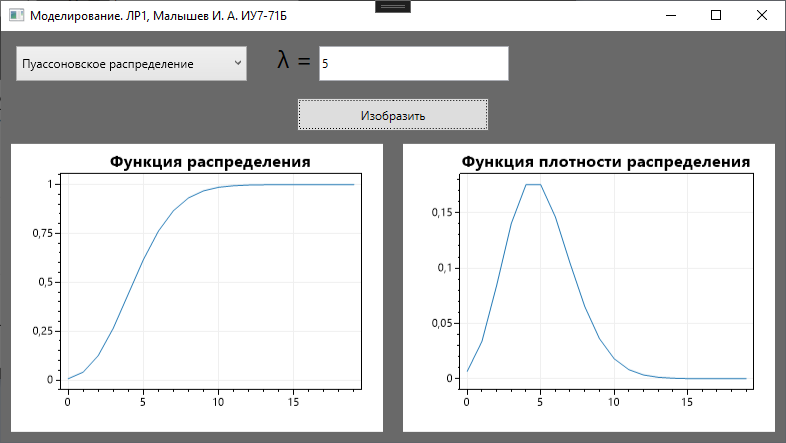
\includegraphics[scale=0.6]{imgs/pois2.png}
	\end{center}
	\caption{Пример работы программы со значением парамера $\lambda = 5$.}
	\label{img:pois2}
\end{figure}

\end{document}